\documentclass[a4paper,11pt]{article}

% packages
% Sprache Deutsch
\usepackage[english,german]{babel}
% 
\author{Baris,Tikir, Leon Dodrimong}
\title{Smart Mirror}

\renewcommand*\contentsname{Inhaltsverzeichnis}
\begin{document}
\maketitle
\newpage
\tableofcontents
\newpage


\section{Grundidee}
\paragraph{Wie wir auf die Idee gekommen sind...}
Auf die eigentliche Idee ist Barsi Tikir eines morgens gekommen als er im Bad stand. Während er sich für den Tag fertig machte und auf seinem Handy noch seine passsende Bahnverbindung raus suchte, dachte er darüber nach, wie praktisch es wäre, wenn man seine Bahnverbindungen nicht mühsam im Handy über die BVG App suchte müsste, sondern diese im irgendwie direkt präsent wäre. Als er darufhin in den Spiegel blickte kam im die Idee.. ein Spiegel  der seine Bahnverbindung anzeigen könnte. Morgens In den Spigel gucken, beim Zähneputzen, Haare machen, usw.... Warum nicht die Zeit auch geich nutzen für ein kleines Update, was in der Welt gerade so passiert oder wann der nächste Bus zur Arbeit fährt. Nach kurzer Recherche fand er auch eine passende Bauanleitung für einen solchen Spiegel. Jedoch gab es neben dem Zusammenbau noch das Problem etwas  sinnvolles auf dem Display anzuzeigen. kleinere Projekt mit Uhrzeit und Wetter gab es bereits, als Beispiele zum nach-programmieren. Aber ein wirkliches System oder fertiges Endprodukt fand er nicht.
\\\
Ein paar Wochen später stieß er auf den Paulaward. Als wir uns trafen, erzählte Baris über die Idee und den Paul Award. Wir fantasierten ein bischen rum und überlegten uns, was denn alles möglich wäre. Zusammen haben wir uns dann rangesetzt und ein Konzept entwickelt, welches möglichst viele Infomationen aus verschiedenen Bereichen anzeigen kann. So entstand die Idee vom "SmartMirror".\\\

\subsection{Spiegel mit integriertem Display}
Ein Spiegel mit integriertem Display ist wohl nichts wirklich neues. Die Idee ist einfach hinter einem Einwegspiegelglass ein Display zu montieren, sodass dieses durch das Glass durch scheint und man dies auf der anderen Seite des Spiegels sehen kann. Von der Anderen Seite wirkt das Galss spiegelnd, wodurch es ganz Normal als Spiegel genutzt werden kann.
\subsection{Gesamtkonzept - eigentliche Idee} 
Unsere eigentliche Idee von uns hinter einen "Spiegel mit integriertem Display" (wird werden ihn im folgenden "SmartMirror" nennen, so wie auch unser Projekt heißt), ist einen System für den SmartMirror zu entwickelt, welches zum einen Benutzerfreundlichkeit(mehr dazu siehe Kapitel \ref{Benutzerfreundlichkeit}) aufweist und zum Anderen mit möglichst vielen Systemen komatibel ist. Wir wollten nicht ein in sich geschlossenes System entwickeln, welches vielleicht gut funktionieren würde, sondern auch ein System, welches bereits vorhandene Dienste nutzen kann. Mehr dazu haben wir im Kapitel \ref{Skalierbarkeit}.
Wir trafen uns meist nach dem Studium und haben uns viele Gedanken darüber gemacht, was der SmartMirror können sollen und über dessen Umsetzung. \\\
Wir stellte einige Grundfunktionen auf die aus unser Sicht wichtig für den SmartMirror wären und welche zusätzlich auch noch sehr praktikabel wären. In diesem Dokument konzentrieren wir uns eher auf die wichtigen Grundfukntionen (Mehr dazu siehe Kapitel \ref{Funktionen} Funktionen).\\\
Danach versuchten wir ein Konzept zu entwickeln, welches allen Anforderungen entspricht. Dabei war es uns sehr wichtig auf den Punkt Skalierbarkeit zu achten.\\\
\begin{figure}[h]
\centering
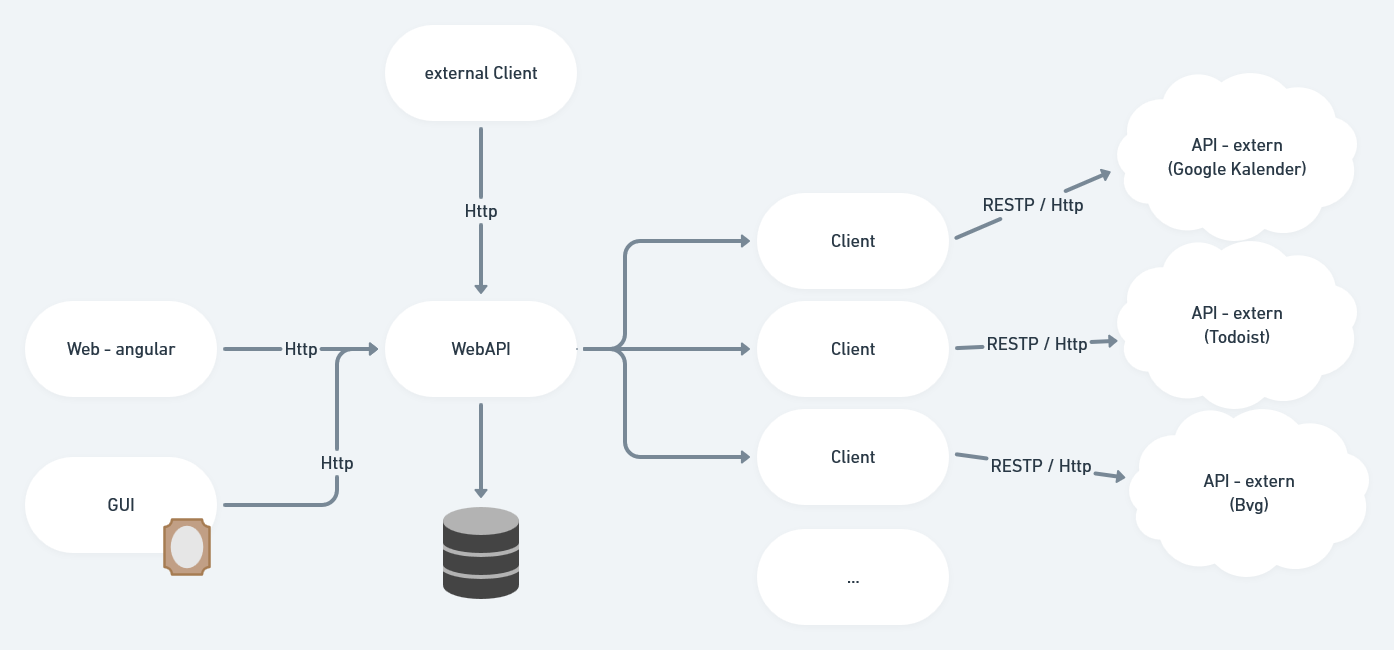
\includegraphics[width=150mm]{pictures/Scalability.png}
\caption{konzeptioneller Aufbau der Software-Komponenten}
\end{figure}\\\
Nach meheren Skizzen und Umgestaltungen kamen wir dann auf diesen Aufbau unserer Software. Auf dem RasperbryPi laufen die folgenden Komponenten: Web - angular, GUI,WebApi, Datenbank und die Clients (mehr zu den einzelnen Komponenten finden sie im Kapitel \ref{Komponenten}). \\\
Die Clients übernehmen die Kommunikation zu den externen Dienst-Anbietern über deren APIs. Die WebAPI organisiert die gesamten anfallenden Daten, wie zum Beispiel: Client-Daten, Benutzerdaten und GUI-Elemente. Auserderm organisiert sie die einzelnen Clients mit deren dazugehörige API und stellt ein eigene API bereit über die Daten abgefragt werden können. Diese API nutzt wiederrum das Frontend, also die GUI Komponente und die Web Komponente. Die GUI ist für die Ansicht auf dem Display hinter dem Glass zuständig. Sie fragt die Daten vom aktuellen Benutzer über die WebAPI ab und formt diese Daten zu einer Ansicht. Die Web Komponente stellt einen Web-Service zur Verfügung, sodass der Benutzer über ein Web-Interface über ein mobiles Endgerät Einstellungen vornehmen kann. Dort kann er Einstllungen bezüglich verschiedener Benutzerkonten und deren Dienste machen. Diese API kann natürlich auch von externen Clients benutzt werden, um zum Beispiel mit eigene SmartHome Produkte mit dem SmartMirror zu interagieren oder den SmartMirror zu steuern.\\\

Um den SmartMirror (RaspberryPi) ins eigene WLAN zu bringen haben wir uns folgende Methodik überlegt. Der RaspberryPi stellt über den integrierten Wifi-chip ein eigenes WLAN zur Verfügung. In dieses muss sich der Benutzer zur Konfiguration einwählen. über ein kleines Web-Interface soll er dann sein WLAN auswählen und das Passwort eingeben oder den SmartMirror über den eigenen WLAN Router freischalten.

\paragraph{Clients}
Die Clients, wobei jeder auf eine spezifische externe API ausgreichtet ist, übernehemen die Kommunikationion zu diesen. Sie kümmern sich um die Authorisierung, Datenabfrage und stellen der WebAPI bestimmte einheitliche Funktionen bereit. Jeder Client muss diese implementieren. Zusätzlich ist der Aufbau der Daten, die zwischen der WebAPI und den Clients übertragen werden, vereinheitlicht und fest definiert. Diese vereinheitlichten Funktionen und Datenmodelle sind in von uns definierten Interfaces beschrieben. Ein Client muss sich an die vorgebenen Funktionen und Datenmodelle halten. Dabei haben wir geguckt, welche Funktionen essentiell wichtig für die Kommunikation sind und wie wir die Daten optimal strukturieren können. (einige Funktionen um nicht zu sehr ins Detail zu gehen zb.: getData(Options):Data, welche Daten von der API und den Bedingungen abfragt; getOptions():Options, welche die Verfügbaren Optionen abfragt; setToken(string):bool, welche den Authorisierungstoken für den jeweiligen Client setzt). Wenn eine neue externe API bereitgestellt werden soll, muss lediglich ein Client programmiert werden, welcher die vorgeschriebenen Funktionen und Datenmodelle implementiert (Interfaces) und die jeweiligen Http-Requests für die API beinhaltet. So kann zu jeder API unter berücksichtigung der Interfaces ein passender Client programmiert werden.\\\
\paragraph{WebAPI}
Die WebAPI übernimmt die 


\subsubsection{Benutzerfreundlichkeit}\label{Benutzerfreundlichkeit}
Die eigentliche Idee dabei ist den Spiegel nicht einfach nur spiegeln zu lassen oder die Uhrzeit anzeigen zu lassen, sondern ihn "smart" zu machen, sodass man ihn praktischen und effizient Nutzen kann. Zudem war uns auch wichtig, dass es \textbf{Benutzerfreundlich} ist, da nicht jeder das Know-How hat sich einen Spiegel für seine Eigenen Bedrüfnisse zusammen zu bauen bzw. zu programmieren. Er sollte einfach und verständlich für jeden sein. Deshalb haben wir auch die in das Konzept die Web Komponente eingefügt und die GUI leicht erweiterbar gestaltet.

\subsubsection{Skalierbarkeit}\label{Skalierbarkeit}
Der SmartMirror ist nicht nur Benutzerfreundlich, sondern ist auch in vielen Richtungen skalierbar.
Wie schon erwähnt, wollten wir die bereits bestehenden Dienste Nutzen. Zum Beispiel hat man seine Kalendereinträge bereits im Google-Kalender eingetragen und hat keine Lust als Kunde alle Daten auf den Kalender des SmartMirrors zu übertragen. Es wäre für den Benutzer leichter auf diese Daten zuzugreifen. \\\
Viele Anbieter von Diensten stellen über das Http-Protokoll API Funktionen für Ihren Dienst bereit. Diese API's nutzt der SmartMirror, um dann die Daten vom dem jeweiligem Dienst abfragen zu können. Dieses Abfragen geschieht in der Client Komponente, auf welche wir näher im Kapitel \ref{Clients} Clients eingehen werden. Dadurch ist das System erweiterbar und hilft sogar beim Vernetzen von anderen Diensten.\\\
Neben der Erweiterbarkeit haben wir auch daran gedacht, eine eigene Schnittstelle zu definieren, sodass andere SmartHome-Produkte sich an den SmartMirror vernetzen können. Diese können dann wie die GUI und Web Komponente, Daten vom SmartMirror abfragen oder senden, sodass es zum Beispiel auch denkbar wäre mehrere SmartHome-Produkte so miteinander zu vernetzen, dass der SmartMirror die Basis bildet.\\\
Im Sinne von Smart Home und Industrie 4.0






\section{Aufbau}
\subsection{Strukturierung}
Notizen: Dagramme und erklärungen der Funktionsweise\\\
\subsection{Materialien}
Der Spiegel besteht aus einem Einwegspiegelglass, welches von einer Seite spiegelt und von der anderen Seite reflektiert. Außerdem haben wir einen Holzrahmen, welcher aus Fassung für das Spiegelglass dient, genutzt. Für die Technik haben wir ein Display für die Anzeigen , ein RasperryPi für die Steuerung und die nötigen Verbindungskabel, wie Spannungsversorgung und Videokabel (HDMI) zur Übertragung der Videosignals zum Display, eingesetzt.\\\
Für die optinalen Erweiterungen würde man je nachdem welches Feature gewünscht ist, noch eine Picamera (für Facerecognition), RasperryPi Bewegungssensor (Bewegungserkennung)\footnote{\textit{ Raspberry Pi Infrarot Bewegungsmelder:} https://www.reichelt.de/raspberry-pi-infrarot-bewegungsmelder-hc-sr501-rpi-hc-sr501-p224216.html?\&nbc=1}, Gesture Sensor (Gestiksteuerung)\footnote{\textit{3D Gesture Tracking Shield for Raspberry Pi:}  http://wiki.seeedstudio.com/3D-Gesture-Tracking-Shield-for-Raspberry-Pi-MGC3130/} oder ein kleines Mikrophone zur Sprachsteuerung \footnote{\textit{Ansteckmikrofon über Klinke:} https://www.amazon.de/dp/B073GJQKL1/ref=psdc\_1384055031\_t1\_B07WQFNVVQ}
\\\\\\
Notizen: Später eintragen welches Raspi Modell, Display, Glass verwendet wurde

\section{Software}
\subsection{Prerequisites}
\begin{itemize}
\item Node.js (Javascript runtime)
\item Angular
\item IDE (Visual Studio Code)
\item Datenbank ()
\end{itemize}

\subsection{Frontend - SmartMirrorWeb}
Wir haben unser Frontend mithilfe von Angular 9. Für uns war dies eine Neue Erfahrung, da wir noch nie zuvor damit gearbeitet haben. Das Frontend soll sich lediglich um die Anzeige der Daten kümmern und folgende Funktionen übernehmen:
\begin{itemize}
\item Daten vom Backend (SmartMirror.WebApi) anfragen
\begin{itemize}
\item alle möglichen Dienste (Widgets)
\item vom User angemeldeten Dienste
\end{itemize}
\item Daten senden
\begin{itemize}
\item Dienst aktivieren/ deaktivieren
\item Benutzereingaben zur Erstellung eines neuen Benutzers
\end{itemize}
\item User zur Anmeldung von weiteren externen Diensten, zur jeweiligen Website weiterleiten\footnote{zum Beispiel: wenn der User den neuen Dienst Google Kalender für sich registrieren möchte, muss er sich auf der Website von Google Kalender anmelden um sich zu zertifizieren. Diese sendet dann die zur Authentifizierung notwendigen Credentials, welche vom Backend gespeichert werden müssen }
\end{itemize} 
\subsection{Backend - SmartMirror.WebApi}
Das Backend besteht aus einer eigens Entwickelten Web API, welche zum einen die Anfragen und Daten vom Frontend (SmartMirror.Web) entgegennimmt und bearbeitet, und zum anderen den Datenaustausch mit der eigenen Datenbank und Kommunikation mit den externen API kommuniziert.\\\
Das Backend besteht zum einen Client-Server. Zum einen stellt er als Server eine eigene API dar, welche vom Frontend genutzt wird. Zum anderen fungiert dieser auch als Client und nutzt die externen API Schnittstellen von Drittanbietern. Besitzt dieser eine extra Komponente, welche auf die interne Datenbank zugreift\\\
\paragraph{Client Funktion}
Da der Smart Mirror möglichst viele externe Features verbinden soll, muss die Schnittstelle zu diesen gut strukturiert werden. Daher haben wir uns dazu entschieden, dass jede externe Kommunikation ihre eigene Komponente bekommet, welche bestimmte Standards (Interfaces) bedient. Somit können auch später leicht neue externe API's eingebunden werden, indem die Kommunikation in einer neuen Komponente implementiert wird. Dort müssen dann nur die vorgegebenen Interfaces definiert sein und dann anschließend bekannt gemacht werden, indem diese in eine interne Liste von allen möglichen externen Diensten eingetragen wird.
\paragraph{Server Funktion}

\paragraph{Kommunikation zur Datenbank}

\section{Erweiterungen}
\subsection{API's}

\begin{itemize}
\item Google Kalender
\item Todoist
\item BVG
\item Wetter
\end{itemize}
\subsection{Hardware}
\begin{itemize}
\item Face Recognition
\item Voice Control
\item Bewegungssensor
\end{itemize}


\section{Über uns}
Wir sind zwei Studenten, Baris Tikir und Leon Dodrimong, von der HTW - Hochschule für
Technik und Wirtschaft Berlin aus dem Fachbereich der Ingenieurwissenschaften und
Technik. 

\section{Anhang}
\subsection{Verweise}


\end{document}